\begin{center}
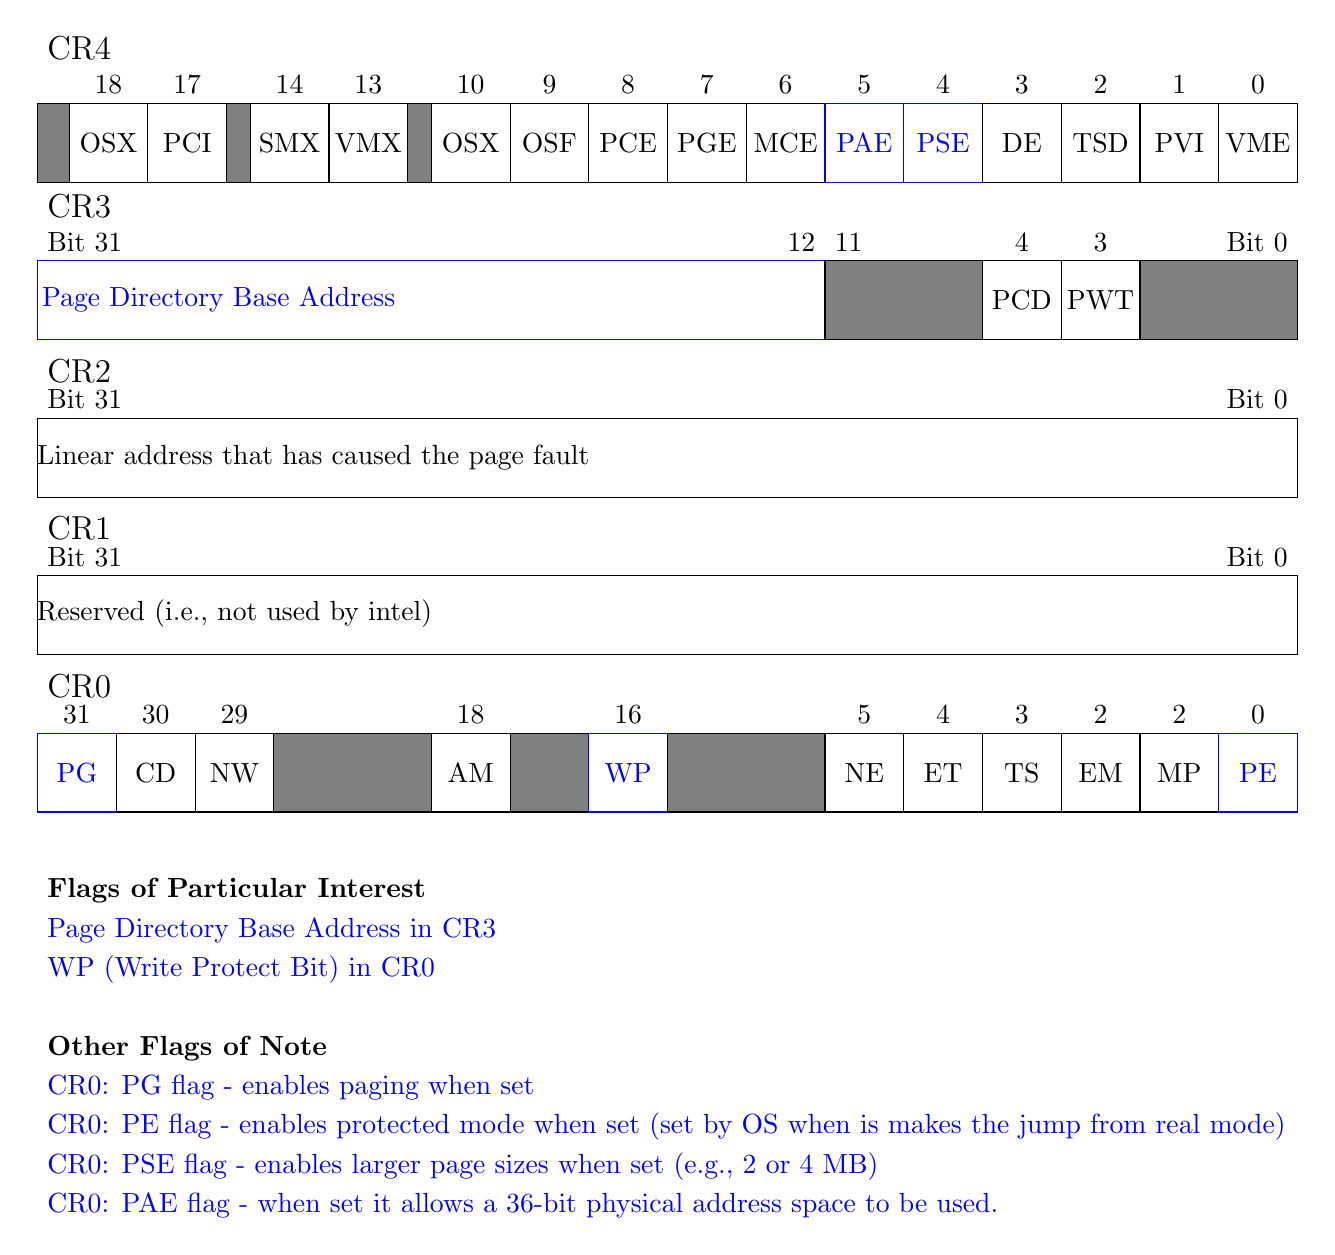
\begin{tikzpicture}
\draw [blue] (0,0) rectangle (1,1) node [pos=0.5] {PG}; \draw node at (0.5,1) [above] {31};
\draw (1,0) rectangle (2,1) node [pos=0.5] {CD}; \draw node at (1.5,1) [above] {30};
\draw (2,0) rectangle (3,1) node [pos=0.5] {NW}; \draw node at (2.5,1) [above] {29};
\draw [fill=gray] (3,0) rectangle (5,1);
\draw (5,0) rectangle (6,1) node [pos=0.5] {AM}; \draw node at (5.5,1) [above] {18};
\draw [fill=gray] (6,0) rectangle (7,1);
\draw [blue] (7,0) rectangle (8,1) node [pos=0.5] {WP}; \draw node at (7.5,1) [above] {16};
\draw [fill=gray] (8,0) rectangle (10,1);
\draw (10,0) rectangle (11,1) node [pos=0.5] {NE}; \draw node at (10.5,1) [above] {5};
\draw (11,0) rectangle (12,1) node [pos=0.5] {ET}; \draw node at (11.5,1) [above] {4};
\draw (12,0) rectangle (13,1) node [pos=0.5] {TS}; \draw node at (12.5,1) [above] {3};
\draw (13,0) rectangle (14,1) node [pos=0.5] {EM}; \draw node at (13.5,1) [above] {2};
\draw (14,0) rectangle (15,1) node [pos=0.5] {MP}; \draw node at (14.5,1) [above] {2};
\draw [blue] (15,0) rectangle (16,1) node [pos=0.5] {PE}; \draw node at (15.5,1) [above] {0};
\draw node at (0,1.6) [right] {\large CR0};

\draw (0,2) rectangle (16,3) node [label={[align=center,xshift=-13.5cm, yshift=-0.9cm] Reserved (i.e., not used by intel)}] {};
\draw node at (0,3) [above right] {Bit 31};
\draw node at (16,3) [above left] {Bit 0};
\draw node at (0,3.6) [right] {\large CR1};

\draw (0,4) rectangle (16,5) node [label={[align=center,xshift=-12.5cm, yshift=-0.9cm] Linear address that has caused the page fault}] {};
\draw node at (0,5) [above right] {Bit 31};
\draw node at (16,5) [above left] {Bit 0};
\draw node at (0,5.6) [right] {\large CR2};

\draw [blue] (0,6) rectangle (10,7) node [label={[align=center,xshift=-7.7cm, yshift=-0.9cm] Page Directory Base Address}] {};
\draw [fill=gray] (10,6) rectangle (12,7);
\draw node at (10,7) [above left] {12}; \draw node at (10,7) [above right] {11};
\draw (12,6) rectangle (13,7) node [pos=0.5] {PCD}; \draw node at (12.5,7) [above] {4};
\draw (13,6) rectangle (14,7) node [pos=0.5] {PWT}; \draw node at (13.5,7) [above] {3};
\draw [fill=gray] (14,6) rectangle (16,7);
\draw node at (0,7) [above right] {Bit 31};
\draw node at (16,7) [above left] {Bit 0};
\draw node at (0,7.7) [right] {\large CR3};

\draw [fill=gray] (0,8) rectangle (0.4,9);
\draw (0.4,8) rectangle (1.4,9) node [pos=0.5] {OSX}; \draw node at (0.9,9) [above] {18};
\draw (1.4,8) rectangle (2.4,9) node [pos=0.5] {PCI}; \draw node at (1.9,9) [above] {17};
\draw [fill=gray] (2.4,8) rectangle (2.7,9);
\draw (2.7,8) rectangle (3.7,9) node [pos=0.5] {SMX}; \draw node at (3.2,9) [above] {14};
\draw (3.7,8) rectangle (4.7,9) node [pos=0.5] {VMX}; \draw node at (4.2,9) [above] {13};
\draw [fill=gray] (4.7,8) rectangle (5,9);
\draw (5,8) rectangle (6,9) node [pos=0.5] {OSX}; \draw node at (5.5,9) [above] {10};
\draw (6,8) rectangle (7,9) node [pos=0.5] {OSF}; \draw node at (6.5,9) [above] {9};
\draw (7,8) rectangle (8,9) node [pos=0.5] {PCE}; \draw node at (7.5,9) [above] {8};
\draw (8,8) rectangle (9,9) node [pos=0.5] {PGE}; \draw node at (8.5,9) [above] {7};
\draw (9,8) rectangle (10,9) node [pos=0.5] {MCE}; \draw node at (9.5,9) [above] {6};
\draw [blue] (10,8) rectangle (11,9) node [pos=0.5] {PAE}; \draw node at (10.5,9) [above] {5};
\draw [blue] (11,8) rectangle (12,9) node [pos=0.5] {PSE}; \draw node at (11.5,9) [above] {4};
\draw (12,8) rectangle (13,9) node [pos=0.5] {DE}; \draw node at (12.5,9) [above] {3};
\draw (13,8) rectangle (14,9) node [pos=0.5] {TSD}; \draw node at (13.5,9) [above] {2};
\draw (14,8) rectangle (15,9) node [pos=0.5] {PVI}; \draw node at (14.5,9) [above] {1};
\draw (15,8) rectangle (16,9) node [pos=0.5] {VME}; \draw node at (15.5,9) [above] {0};
\draw node at (0,9.7) [right] {\large CR4};

\draw node at (0,-1) [right] {\textbf{Flags of Particular Interest}};
\draw [blue] node at (0,-1.5) [right] {Page Directory Base Address in CR3};
\draw [blue] node at (0,-2) [right] {WP (Write Protect Bit) in CR0};
\draw node at (0,-3) [right] {\textbf{Other Flags of Note}};
\draw [blue] node at (0,-3.5) [right] {CR0: PG flag - enables paging when set};
\draw [blue] node at (0,-4) [right] {CR0: PE flag - enables protected mode when set (set by OS when is makes the jump from real mode)};
\draw [blue] node at (0,-4.5) [right] {CR0: PSE flag - enables larger page sizes when set (e.g., 2 or 4 MB)};
\draw [blue] node at (0,-5) [right] {CR0: PAE flag - when set it allows a 36-bit physical address space to be used.};
\end{tikzpicture}
\end{center}